\begin{exercises} 
\item Consider the graph of $y = f(x)$ provided in Figure~\ref{F:1.3.Ez1}.
	\ba
		\item On the graph of $y = f(x)$, sketch and label the following quantities:
		\begin{itemize}
			\item the secant line to $y = f(x)$ on the interval $[-3,-1]$ and the secant line to $y = f(x)$ on the interval $[0,2]$.
			\item the tangent line to $y = f(x)$ at $x = -3$ and the tangent line to $y = f(x)$ at $x = 0$.
		\end{itemize}
\begin{figure}[h]
  \begin{center}
 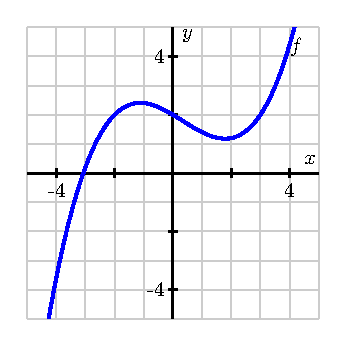
\includegraphics{figures/1_3_Ez1.eps}    \end{center}
   \caption{Plot of $y = f(x)$.} \label{F:1.3.Ez1}
\end{figure}
		\item What is the approximate value of the average rate of change of $f$ on $[-3,-1]$?  On $[0,2]$?  How are these values related to your work in (a)?
		\item What is the approximate value of the instantaneous rate of change of $f$ at $x = -3$?  At $x = 0$?  How are these values related to your work in (a)?

	\ea	
	
\begin{exerciseSolution}
\end{exerciseSolution}
\item For each of the following prompts, sketch a graph on the provided axes in Figure~\ref{F:1.3.Ez2} of a function that has the stated properties.
  \ba
  	\item $y = f(x)$ such that 
	\begin{itemize}
		\item the average rate of change of $f$ on $[-3,0]$ is $-2$ and the average rate of change of $f$ on $[1,3]$ is 0.5, and
		\item the instantaneous rate of change of $f$ at $x = -1$ is $-1$ and the instantaneous rate of change of $f$ at $x = 2$ is 1. 
	\end{itemize}
	\item $y = g(x)$ such that
	\begin{itemize}
		\item $\frac{g(3)-g(-2)}{5} = 0$ and $\frac{g(1)-g(-1)}{2} = -1$, and
		\item $g'(2) = 1$ and $g'(-1) = 0$
	\end{itemize}
\begin{figure}[h]
  \begin{center}
 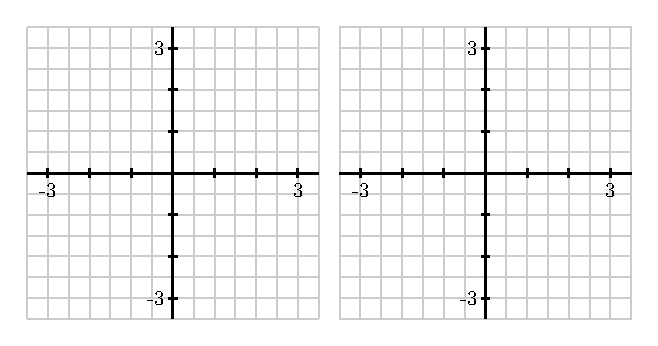
\includegraphics{figures/1_2_Ez3.eps} %\ \  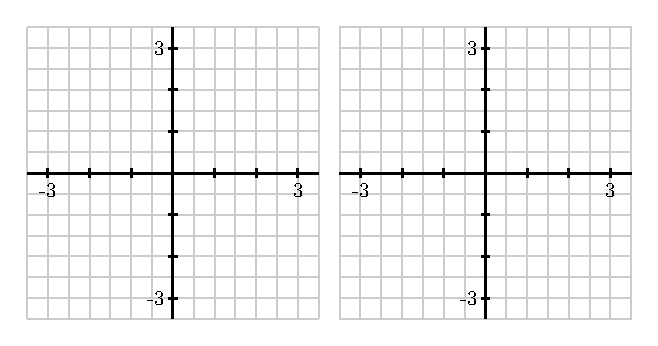
\includegraphics{figures/1_2_Ez3.eps}
   \end{center}
   \caption{Axes for plotting $y = f(x)$ in (a) and $y = g(x)$ in (b).} \label{F:1.3.Ez2}
\end{figure}
  \ea

\item Suppose that the population, $P$, of China (in billions) can be approximated by the function $P(t) = 1.15(1.014)^t$ where $t$ is the number of years since the start of 1993.
   \ba
   	\item According to the model, what was the total change in the population of China between January 1, 1993 and January 1, 2000?  What will be the average rate of change of the population over this time period?  Is this average rate of change greater or less than the instantaneous rate of change of the population on January 1, 2000?  Explain and justify, being sure to include proper units on all your answers.
	\item According to the model, what is the average rate of change of the population of China in the ten-year period starting on January 1, 2012?
	\item Write an expression involving limits that, if evaluated, would give the exact instantaneous rate of change of the population on today's date.  Then estimate the value of this limit (discuss how you chose to do so) and explain the meaning (including units) of the value you have found.
	\item Find an equation for the tangent line to the function $y = P(t)$ at the point where the $t$-value is given by today's date.  
   \ea

\item The goal of this problem is to compute the value of the derivative at a point for several different functions, where for each one we do so in three different ways, and then to compare the results to see that each produces the same value.

For each of the following functions, use the limit definition of the derivative to compute the value of $f'(a)$ using three different approaches:  strive to use the algebraic approach first (to compute the limit exactly), then test your result using numerical evidence (with small values of $h$), and finally plot the graph of $y = f(x)$ near $(a,f(a))$ along with the appropriate tangent line to estimate the value of $f'(a)$ visually.  Compare your findings among all three approaches.

	\ba
		\item $f(x) = x^2 - 3x$, $a = 2$
		\item $f(x) = \frac{1}{x}$, $a = 1$
		\item $f(x) = \sin(x)$, $a = \frac{\pi}{2}$
		\item $f(x) = \sqrt{x}$, $a = 1$
		\item $f(x) = 2 - |x-1|$, $a = 1$
	\ea

\end{exercises}
\afterexercises